\chapter{Apron design}
	\section{Pavement}
		In order to calculate the thickness of the rigid pavement, the following parameters are needed:
		
		- The flexural resistance of the cement in psi. 
		
		- The coefficient of resistance of the cement that is going to be placed in the pavement (K).
		
		- The maximum takeoff weight of the critical aircraft that is going to operate on the apron.
		
		- The number of operations a year of the plane.
		
		The critical aircraft is the B737 due to the large amount of operations every done a year, more than 40\% of the total operations in comparison with the less than a \% done by de 777. Another possible candidate is the Airbus A320, however, it has been discarded due to the fact that the B737 has a higher MTOW.
		
		Moving into the thickness calculation, using the flexural resistance of 600psi, a parameter K of 180psi, a MTOW of 170.000lbs, a number of operations a year of 25.000 and introducing those inputs in the following graph taken from the FAA: 
		
		\begin{figure}[H]
			\centering
			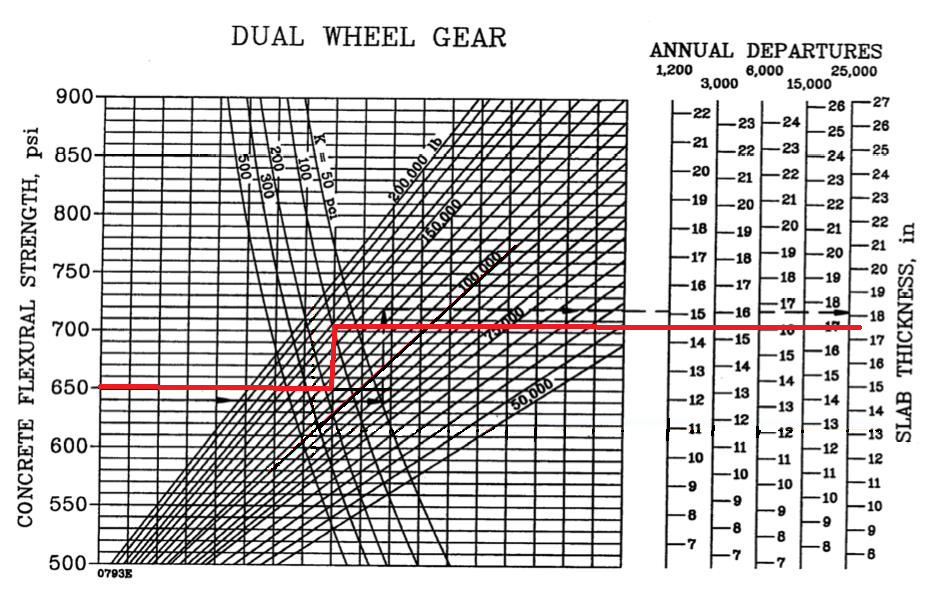
\includegraphics[clip, trim=0cm 0cm 0cm 0cm, width=0.95\textwidth]{./images/pavement/apron/thickness1}
			\caption{Thickness of the cement slab.}
			\label{} %per denotar una referencia
		\end{figure}
	
	The value of thickness obtained is 17,5in, which are 44cm. However, this thickness has to be corrected by the total number of operations done in the apron. Using the same equation used in the calculations of the runway's pavement:
	
	\[T_{total} = T_t * (1+0,133*\log(\dfrac{N}{25.000})) = 44 * (1+0,133*\log(\dfrac{270.000}{25.000}))= 51cm\]
	
	The final value of the slab's thickness obtained after the correction is \(T_{total}=51cm\).